\documentclass[12pt,addpoints]{repaso}
\grado{2}
\nivel{Secundaria}
\cicloescolar{2024-2025}
\materia{Matemáticas 2 \normalfont \color{darkgray} \\[-0.2em]\small con adecuación curricular a Matemáticas 1$^\circ$ de Secundaria}
\unidad{1}
\title{Repaso para el examen de la Unidad}
\aprendizajes{
      \item Convierte fracciones decimales a notación decimal y viceversa. Aproxima algunas fracciones no decimales usando la notación decimal. 
      \item Ordena fracciones y números decimales.
      \item Resuelve problemas de suma y resta con números enteros, fracciones y decimales positivos y negativos.
      \item Resuelve problemas de multiplicación con fracciones y decimales y de división con decimales.
}
\author{Melchor Pinto, J.C.}
\begin{document}
\INFO%
\begin{questions}
      \section*{\ifprintanswers{Cálculos numéricos}\else{}\fi}

      \questionboxed[10]{Realiza las siguientes operaciones de \textit{cálculo numérico}:

            \begin{parts}
                  \begin{multicols}{2}
                        \subsection*{\ifprintanswers{Suma de números}\else{}\fi}
                        \part $\dfrac{5}{6}+\dfrac{3}{8}=$ \fillin[$1\dfrac{5}{24}$][0in]
                        \part $0.5+0.25+0.125=$ \fillin[$0.875$][0in]
                        \part $\dfrac{1}{2}+\dfrac{2}{5}=$ \fillin[$\dfrac{9}{10}$][0in]
                        \part $1.25+0.5+0.25=$ \fillin[$2$][0in]
                        \subsection*{\ifprintanswers{Multiplicación de números}\else{}\fi}
                        \part $9.27\times 5.4=$ \fillin[$50.058$][0in]
                        \part $0.5\times 0.25=$ \fillin[$0.125$][0in]
                        \part $0.5\times 0.25\times 0.125=$ \fillin[$0.015625$][0in]
                        \part $2.5\times 0.4=$ \fillin[$1$][0in]
                        \subsection*{\ifprintanswers{Resta de números}\else{}\fi}
                        \part $\dfrac{1}{2}-\dfrac{2}{5}=$ \fillin[$\dfrac{1}{10}$][0in]
                        \part $1.25-0.5-0.25=$ \fillin[$0.5$][0in]
                        \part $\dfrac{5}{6}-\dfrac{3}{4}=$ \fillin[$-\dfrac{1}{12}$][0in]
                        \part $0.5-0.25-0.125=$ \fillin[$0.125$][0in]
                        \subsection*{\ifprintanswers{División de números}\else{}\fi}
                        \part $622.21\divisionsymbol 115=$ \fillin[$5.41$][0in]
                        \part $0.5\divisionsymbol 0.25=$ \fillin[$2$][0in]
                        \part $5\divisionsymbol 0.5=$ \fillin[$10$][0in]
                        \part $\dfrac{1}{2}\divisionsymbol\dfrac{2}{5}=$ \fillin[$\dfrac{5}{4}$][0in]
                        \subsection*{\ifprintanswers{Resolución de problemas}\else{}\fi}
                        \part Si un dólar equivale a 19 pesos. ¿Cuántos dólares serán 1634 pesos? \fillin[$1634\divisionsymbol 19 =$ 86 dólares][0in]
                        % \part Los alumnos de secundaria van a comprar un balón de fútbol que cuesta 437.50 pesos. Si son un total de 35 alumnos, ¿con cuánto dinero debe cooperar cada alumno? \fillin[$437.50\divisionsymbol 35 =$ 12.5 pesos][0in]
                        \part Un automóvil viaja a 112.4 kilómetros por hora en una carretera. ¿Qué distancia recorre en 4 horas? \fillin[$112.4\times 4 =$ 449.6 kilómetros][0in]
                  \end{multicols}
                  % 
            \end{parts}
      }

      \section*{\ifprintanswers{Fracciones}\else{}\fi}

      \subsection*{\ifprintanswers{Clasificación de fracciones}\else{}\fi}

      \questionboxed[8]{Clasifica las siguientes fracciones en propias, impropias o mixtas:
            \begin{multicols}{2}
                  \begin{parts}
                        \part $\dfrac{5}{6}=$ \fillin[Propia][1in]   \\
                        \part $5\dfrac{5}{11}=$ \fillin[Mixta][1in]  \\
                        \part $\dfrac{7}{3}=$ \fillin[Impropia][1in] \\
                        \part $\dfrac{3}{4}=$ \fillin[Propia][1in]   \\
                        \part $1\dfrac{2}{3}=$ \fillin[Mixta][1in]   \\
                        \part $\dfrac{7}{5}=$ \fillin[Impropia][1in] \\
                        \part $\dfrac{7}{8}=$ \fillin[Propia][1in] \\
                        \part $3\dfrac{2}{9}=$ \fillin[Mixta][1in]   \\
                        \part $\dfrac{3}{2}=$ \fillin[Impropia][1in]   \\
                        \part $4\dfrac{1}{4}=$ \fillin[Mixta][1in] \\
                  \end{parts}
            \end{multicols}
      }

      \subsection*{\ifprintanswers{Representación de fracciones}\else{}\fi}
      \questionboxed[4]{Escribe sobre la línea la fracción que representa cada imagen:
            \begin{multicols}{2}
                  \begin{parts}
                        \part 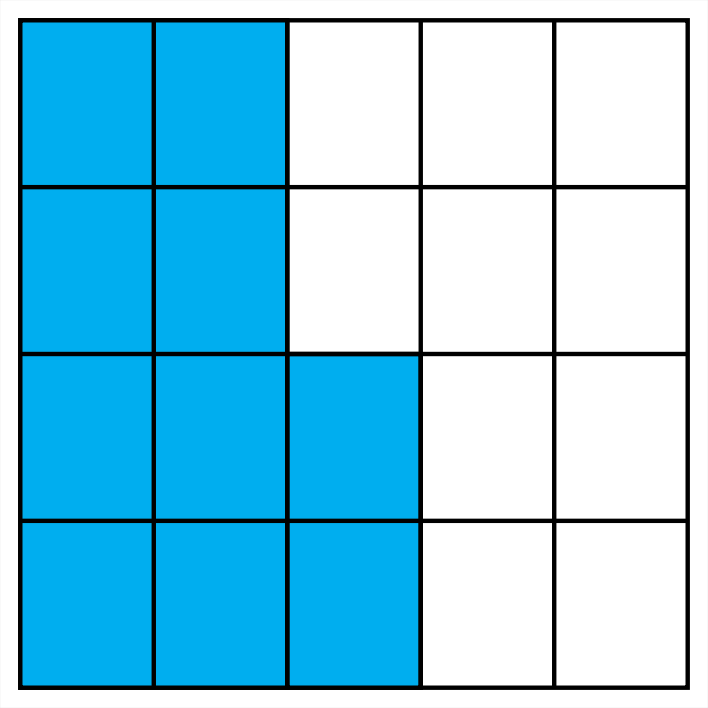
\includegraphics[width=80px]{../images/imagen_frac01.png} \fillin[$\dfrac{10}{20}$][1in]
                        \part 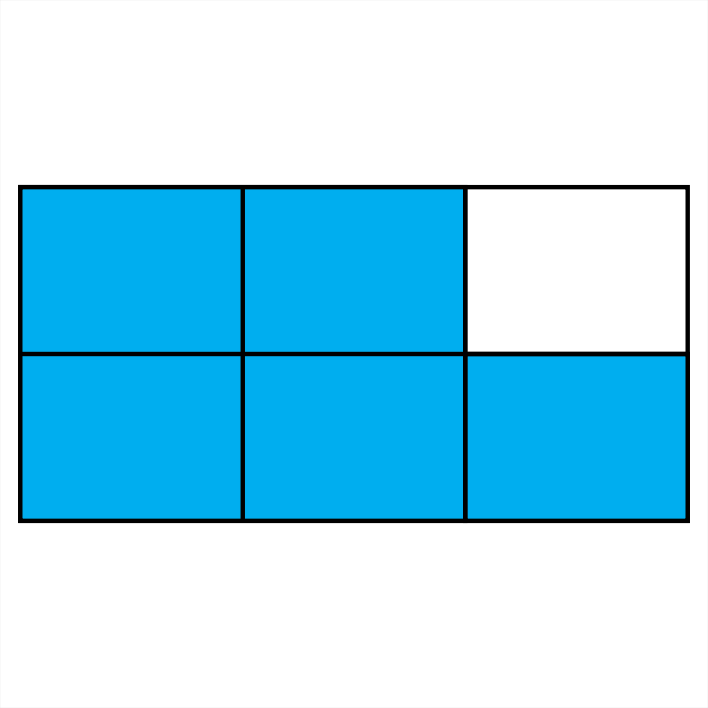
\includegraphics[width=80px]{../images/imagen_frac02.png} \fillin[$\dfrac{5}{6}$][1in]
                        \part 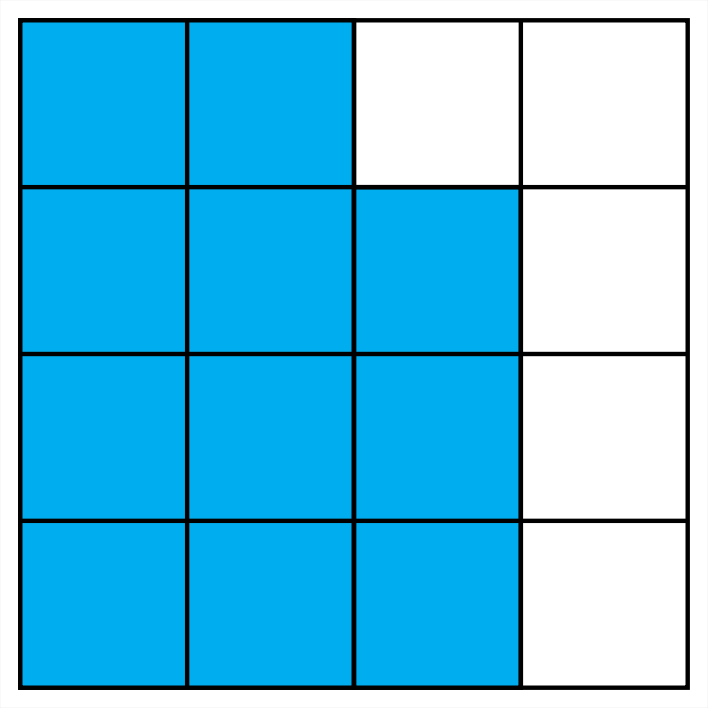
\includegraphics[width=80px]{../images/imagen_frac03.png} \fillin[$\dfrac{11}{16}$][1in]
                        \part 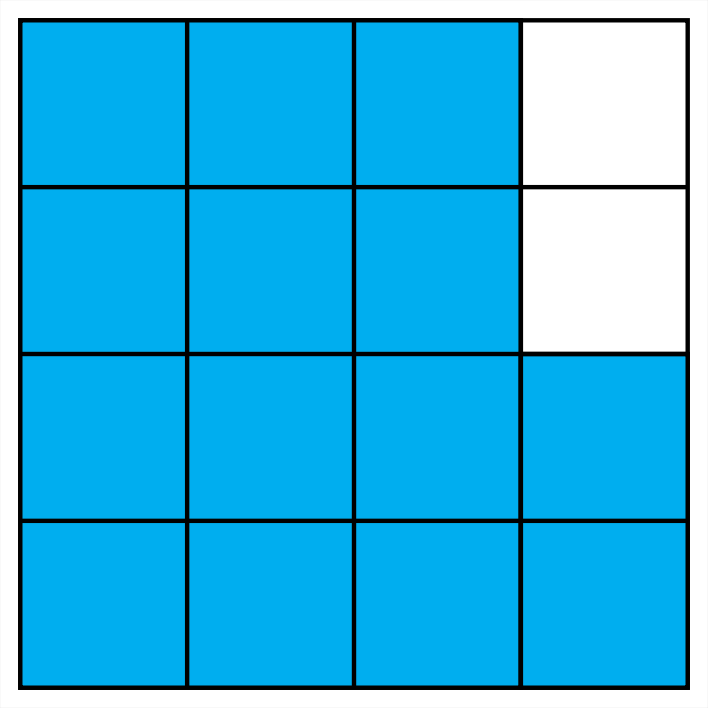
\includegraphics[width=80px]{../images/imagen_frac04.png} \fillin[$\dfrac{14}{16}$][1in]
                        % \part 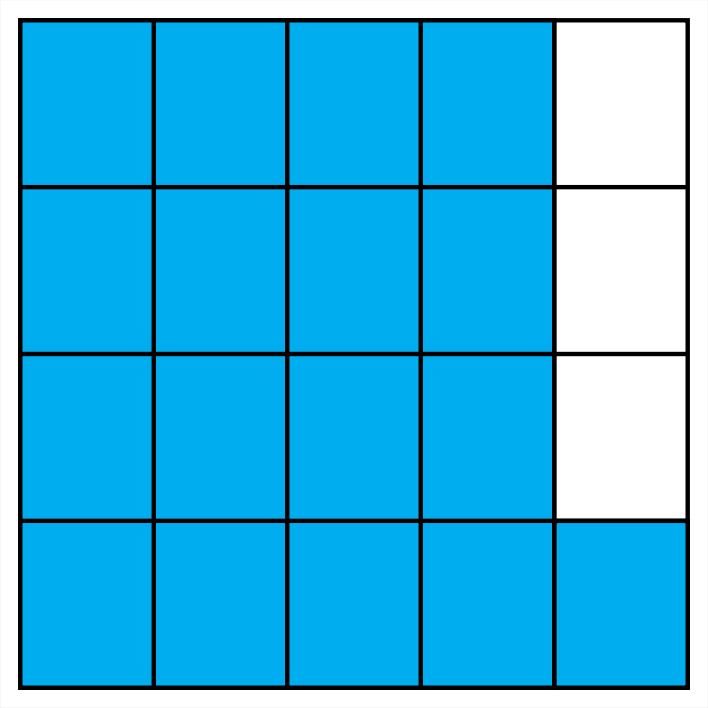
\includegraphics[width=100px]{../images/imagen_frac05.png} \fillin[$\dfrac{10}{20}$][1in]
                        % \part 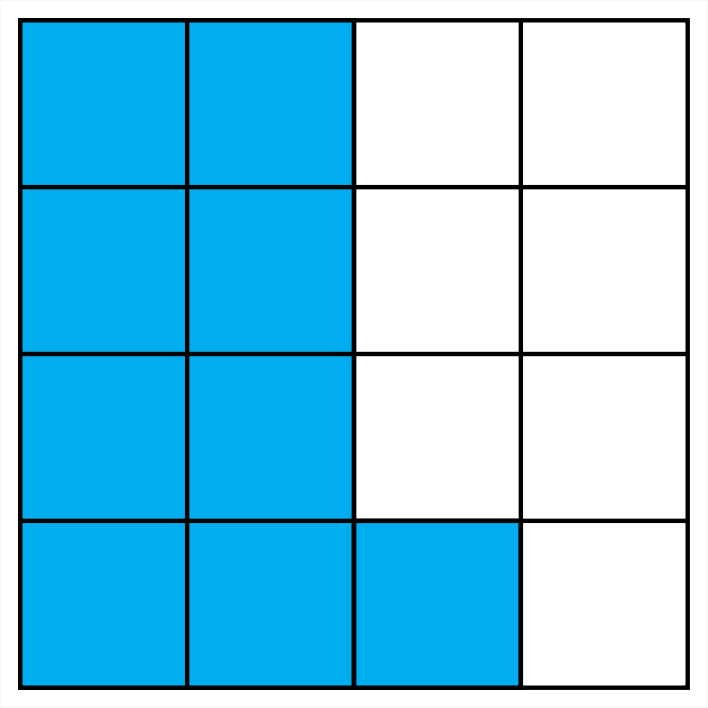
\includegraphics[width=100px]{../images/imagen_frac06.png} \fillin[$\dfrac{10}{20}$][1in]
                        \part 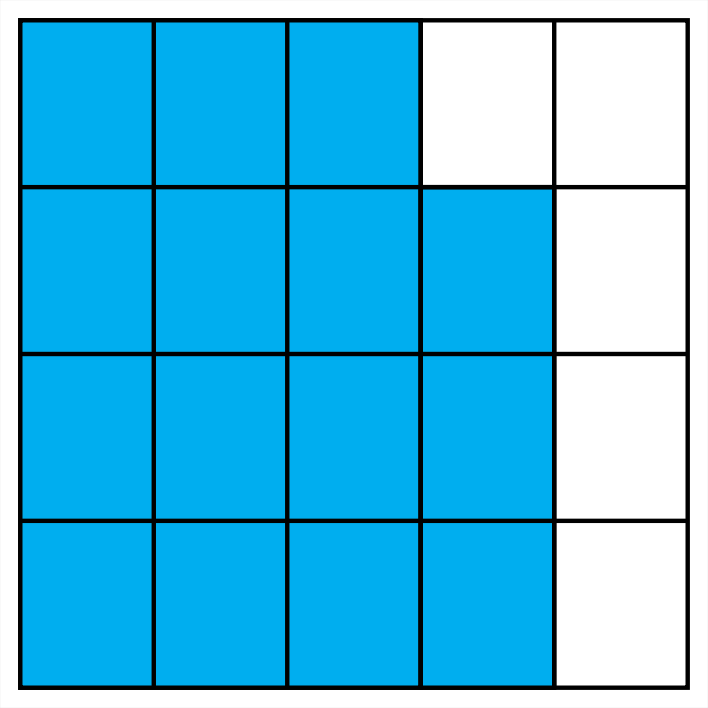
\includegraphics[width=80px]{../images/imagen_frac07.png} \fillin[$\dfrac{15}{20}$][1in]
                        \part 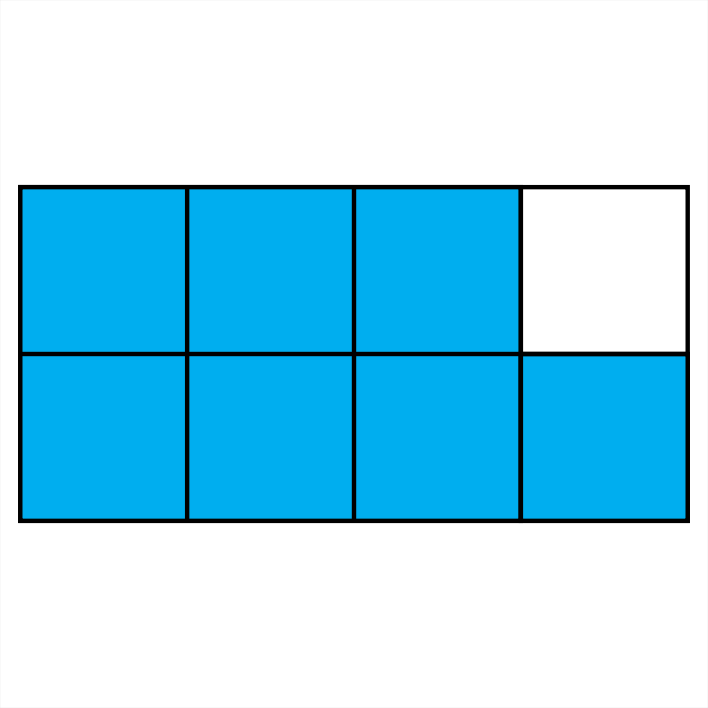
\includegraphics[width=80px]{../images/imagen_frac08.png} \fillin[$\dfrac{7}{8}$][1in]
                        % \part 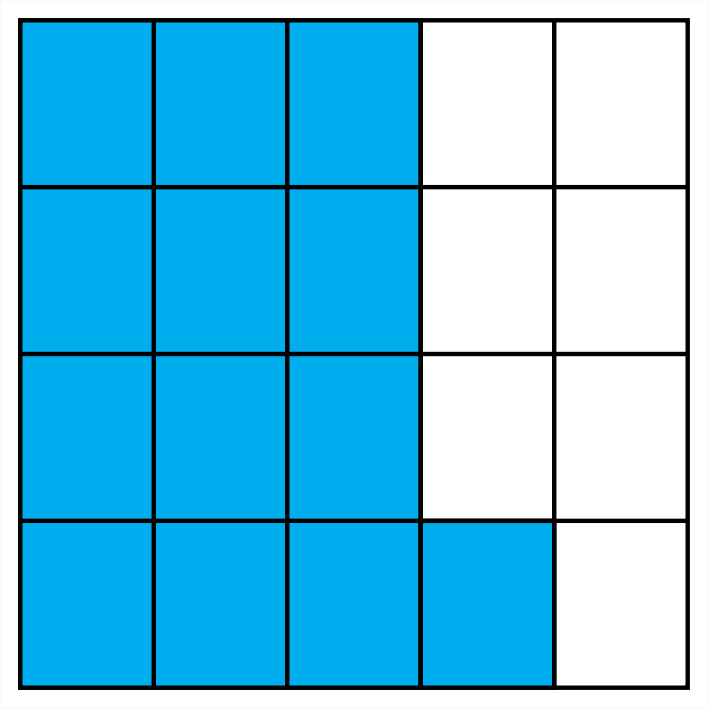
\includegraphics[width=100px]{../images/imagen_frac09.png} \fillin[$\dfrac{10}{20}$][1in]
                        % \part 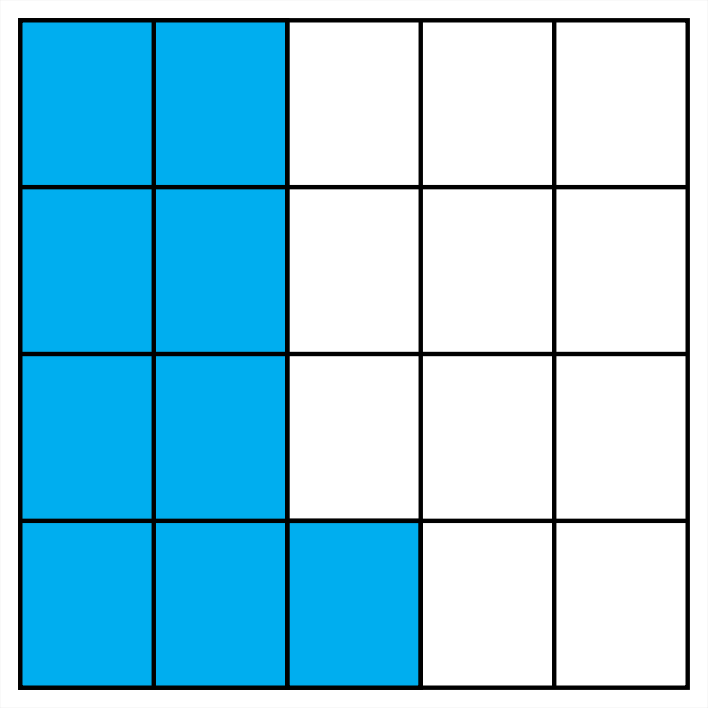
\includegraphics[width=100px]{../images/imagen_frac10.png} \fillin[$\dfrac{10}{20}$][1in]
                  \end{parts}
            \end{multicols}
      }

      \subsection*{\ifprintanswers{Nombre de fracciones}\else{}\fi}

      \questionboxed[4]{Escribe la fracción que corresponda en cada inciso:
            \begin{parts}
                  \part ¿Cómo se escribe numéricamente la fracción \textbf{ocho quintos}?    \fillin[$\dfrac{8}{5}$][0in]  \\
                  \part ¿Cómo se escribe numéricamente la fracción \textbf{seis onceavos}?   \fillin[$\dfrac{6}{11}$][0in] \\
                  \part ¿Cómo se escribe numéricamente la fracción \textbf{dos séptimos}?    \fillin[$\dfrac{2}{7}$][0in]  \\
                  \part ¿Cómo se escribe numéricamente la fracción \textbf{once medios}?     \fillin[$\dfrac{11}{2}$][0in] \\
                  \part ¿Cómo se escribe numéricamente la fracción \textbf{diez décimos}?    \fillin[$\dfrac{10}{10}$][0in]\\
            \end{parts}
      }

      \subsection*{\ifprintanswers{Fracciones en la recta numérica}\else{}\fi}

      \questionboxed[4]{Escribe la fracción que representa el punto en la recta numérica
            \begin{multicols}{2}
                  \begin{parts}
                        \part 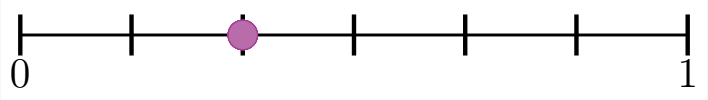
\includegraphics[width=150px]{../images/recta_num_frac01.png} \\ \fillin[$\dfrac{2}{6}$][1in]
                        \part 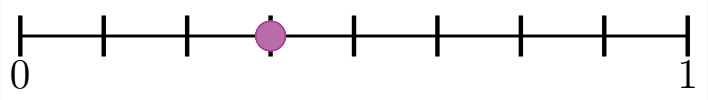
\includegraphics[width=150px]{../images/recta_num_frac03.png} \\ \fillin[$\dfrac{3}{8}$][1in]
                        \part 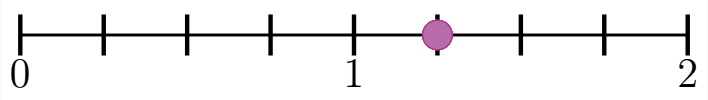
\includegraphics[width=150px]{../images/recta_num_frac04.png} \\ \fillin[$\dfrac{5}{4}$][1in]
                        \part 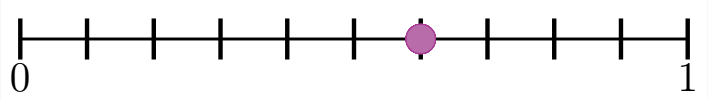
\includegraphics[width=150px]{../images/recta_num_frac05.png} \\ \fillin[$\dfrac{6}{10}$][1in]
                        \part 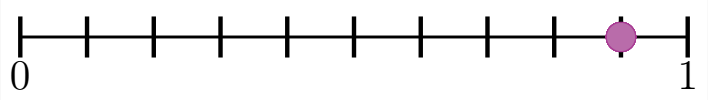
\includegraphics[width=150px]{../images/recta_num_frac06.png} \\ \fillin[$\dfrac{9}{10}$][1in]
                        \part 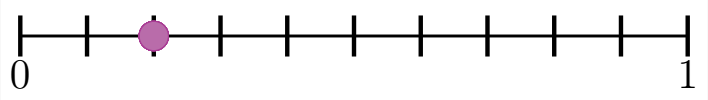
\includegraphics[width=150px]{../images/recta_num_frac02.png} \\ \fillin[$\dfrac{2}{10}$][1in]
                        \part 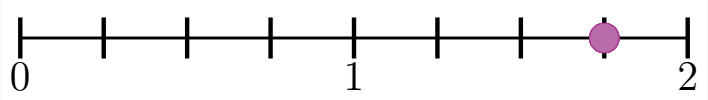
\includegraphics[width=150px]{../images/recta_num_frac07.png} \\ \fillin[$\dfrac{7}{4}$][1in]
                        \part 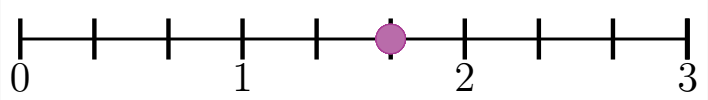
\includegraphics[width=150px]{../images/recta_num_frac08.png} \\ \fillin[$\dfrac{5}{3}$][1in]
                        \part 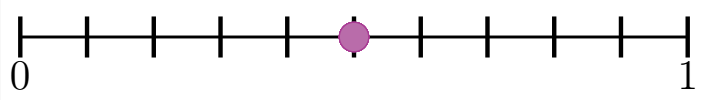
\includegraphics[width=150px]{../images/recta_num_frac09.png} \\ \fillin[$\dfrac{5}{10}$][1in]
                        \part 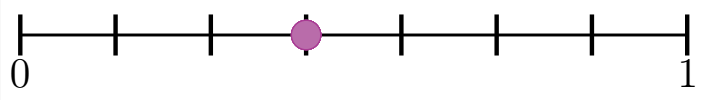
\includegraphics[width=150px]{../images/recta_num_frac10.png} \\ \fillin[$\dfrac{3}{7}$][1in]
                  \end{parts}
            \end{multicols}
      }
      \subsection*{\ifprintanswers{Conversión de fracciones}\else{}\fi}

      \questionboxed[4]{Convierte la siguientes fracciones impropias a mixtas:
            \begin{multicols}{3}
                  \begin{parts}\large
                        \part $\dfrac{13}{3}= $ \fillin[$4\dfrac{1}{3}$][0in]
                        \part $\dfrac{63}{10}= $ \fillin[$6\dfrac{3}{10}$][0in]
                        \part $\dfrac{51}{5}= $ \fillin[$10\dfrac{1}{5}$][0in]
                  \end{parts}
            \end{multicols}
      }

      \section*{\ifprintanswers{Fracciones, M.C.M. y M.C.D.}\else{}\fi}

      \subsection*{\ifprintanswers{Comparación de fracciones}\else{}\fi}

      \questionboxed[8]{Compara las siguientes fracciones usando los signos mayor que (>), menor que (<) o igual (=):
            \begin{multicols}{3}
                  \begin{parts}\large
                        \part $\dfrac{4}{3}$ \fillin[$>$][0.5in] $\dfrac{5}{4}$\\[0.5em]
                        \part $\dfrac{1}{3}$ \fillin[$=$][0.5in] $\dfrac{3}{9}$\\[0.5em]
                        \part $\dfrac{2}{3}$ \fillin[$<$][0.5in] $\dfrac{3}{2}$\\[0.5em]
                        \part $\dfrac{3}{4}$ \fillin[$>$][0.5in] $\dfrac{2}{3}$\\[0.5em]
                        \part $\dfrac{5}{6}$ \fillin[$>$][0.5in] $\dfrac{4}{5}$\\[0.5em]
                        \part $\dfrac{1}{3}$ \fillin[$<$][0.5in] $\dfrac{2}{5}$\\[0.5em]
                  \end{parts}
            \end{multicols}
      }
      \subsection*{\ifprintanswers{Fracciones equivalentes}\else{}\fi}
      \questionboxed[8]{Indica si las siguientes fracciones son equivalentes o no:
            \begin{multicols}{2}
                  \begin{parts}
                        \part $\dfrac{4}{5}=\dfrac{8}{10}$\qquad
                        \begin{oneparcheckboxes}
                              \CorrectChoice Sí
                              \choice No
                        \end{oneparcheckboxes}

                        \part $\dfrac{1}{8}=\dfrac{4}{16}$\qquad
                        \begin{oneparcheckboxes}
                              \choice Sí
                              \CorrectChoice No
                        \end{oneparcheckboxes}

                        \part $\dfrac{1}{5}=\dfrac{5}{10}$\qquad
                        \begin{oneparcheckboxes}
                              \choice Sí
                              \CorrectChoice No
                        \end{oneparcheckboxes}

                        \part $\dfrac{1}{10}=\dfrac{3}{30}$\qquad
                        \begin{oneparcheckboxes}
                              \CorrectChoice Sí
                              \choice No
                        \end{oneparcheckboxes}

                        \part $\dfrac{1}{4}=\dfrac{2}{4}$\qquad
                        \begin{oneparcheckboxes}
                              \choice Sí
                              \CorrectChoice No
                        \end{oneparcheckboxes}

                        \part $\dfrac{3}{2}=\dfrac{12}{8}$\qquad
                        \begin{oneparcheckboxes}
                              \CorrectChoice Sí
                              \choice No
                        \end{oneparcheckboxes}

                        \part $\dfrac{3}{6}=\dfrac{1}{3}$\qquad
                        \begin{oneparcheckboxes}
                              \choice Sí
                              \CorrectChoice No
                        \end{oneparcheckboxes}

                        \part $\dfrac{18}{12}=\dfrac{9}{4}$\qquad
                        \begin{oneparcheckboxes}
                              \choice Sí
                              \CorrectChoice No
                        \end{oneparcheckboxes}
                  \end{parts}
            \end{multicols}
      }

      \subsection*{\ifprintanswers{M.C.D y M.C.M}\else{}\fi}
      \questionboxed[4]{Calcula lo que se te pide en cada inciso:
            \begin{parts}
                  \part Encuentra el máximo común divisor de 33 y 121. \fillin[$\text{mcd}(33,121)=11$][0in]
                  \part Encuentra el mínimo común múltiplo de 12, 15 y 18. \fillin[$\text{mcm}(12,15,18)=180$][0in]
                  \part Encuentra el mínimo común múltiplo de 2, 3 y 4. \fillin[$\text{mcm}(2,3,4)=12$][0in]
                  \part Encuentra el máximo común divisor de 12, 15 y 18. \fillin[$\text{mcd}(12,15,18)=3$][0in]
            \end{parts}
      }

      \subsection*{\ifprintanswers{Simplificación de fracciones}\else{}\fi}
      \questionboxed[4]{Simplifica a su mínima expresión la siguiente fracción usando el máximo común divisor
            \begin{multicols}{2}
                  \begin{parts}\large
                        \part $\dfrac{6}{42}=$ \fillin[$\dfrac{1}{7}$][0in]
                        \part $\dfrac{12}{18}=$ \fillin[$\dfrac{2}{3}$][0in]
                        \part $\dfrac{15}{30}=$ \fillin[$\dfrac{1}{2}$][0in]
                        \part $\dfrac{24}{36}=$ \fillin[$\dfrac{2}{3}$][0in]
                        \part $\dfrac{8}{64}=$ \fillin[$\dfrac{1}{8}$][0in]
                        \part $\dfrac{16}{24}=$ \fillin[$\dfrac{2}{3}$][0in]
                  \end{parts}
            \end{multicols}
      }

      \subsection*{\ifprintanswers{Resolución de problemas}\else{}\fi}

      \questionboxed[6]{\large María y Jorge tienen 45 bolas blancas, 15 bolas azules y 90 bolas rojas y quieren hacer el mayor número de collares iguales sin que sobre ninguna bola. ¿Cuántos collares iguales pueden hacer?
            \begin{solutionbox}{4cm}
                  Se calcula el M.C.D.$(45,15,90) = 15$.\\
                  Por lo tanto, se pueden hacer 15 collares.
            \end{solutionbox}
      }

      \section*{\ifprintanswers{Números decimales}\else{}\fi}

      \subsection*{\ifprintanswers{Ubicación en la recta numérica}\else{}\fi}

      \questionboxed[4]{Escribe el número que representa el punto indicado en la recta numérica de cada uno de los siguientes incisos.

            \begin{multicols}{2}
                  \begin{parts}
                        %\part 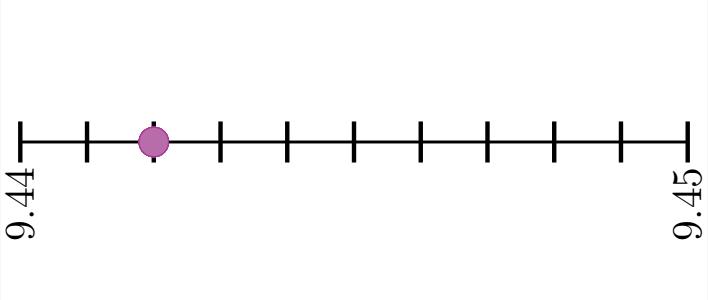
\includegraphics[width=150px]{../images/recta_num_9.442.png}\\[-0.5em]  \fillin[$9.44$][1.5in]
                        \part 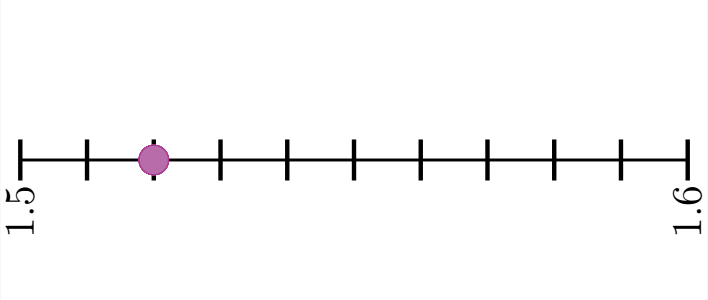
\includegraphics[width=160px]{../images/recta_num_1.52.png} \\[-0.5em] \fillin[$1.52$][1.5in]
                        \part 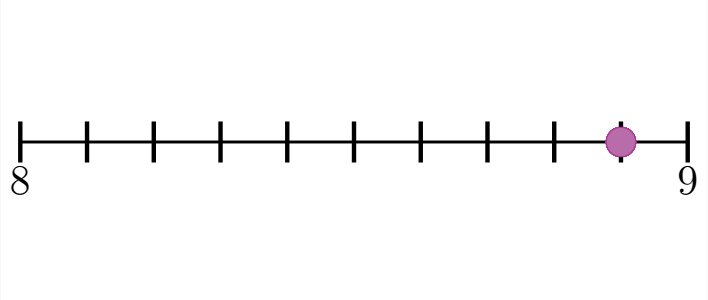
\includegraphics[width=160px]{../images/recta_num_8.9.png}  \\[-0.5em]  \fillin[$8.9$][1.5in]
                        \part 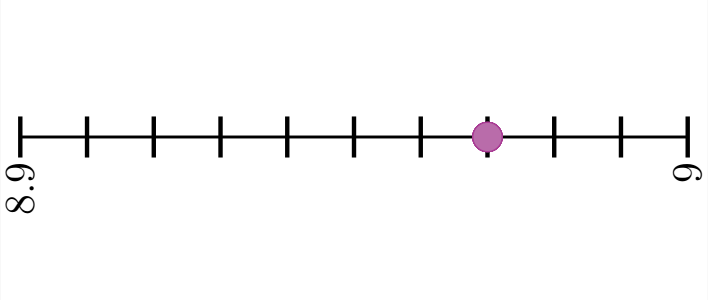
\includegraphics[width=160px]{../images/recta_num_8.97.png} \\[-0.5em]  \fillin[$8.97$][1.5in]
                        \part 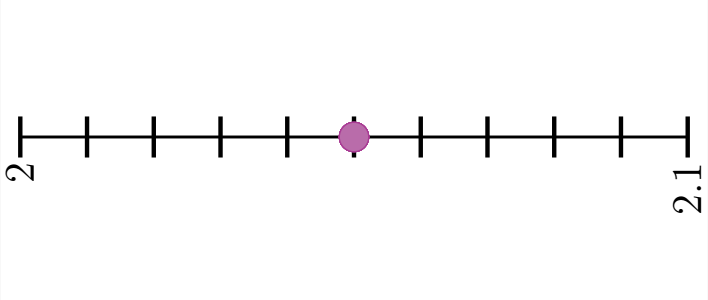
\includegraphics[width=160px]{../images/recta_num_2.05.png} \\[-0.5em]  \fillin[$2.05$][1.5in]
                  \end{parts}
            \end{multicols}
      }

      \subsection*{\ifprintanswers{Porcentajes a decimal}\else{}\fi}

      \questionboxed[4]{Escribe el número decimal que representa cada porcentaje:

            \begin{multicols}{2}
                  \begin{parts}
                        \part Convierte 50\% a un número decimal. \fillin[$0.5$][0.4in]
                        \part Convierte 25\% a un número decimal. \fillin[$0.25$][0.4in]
                        \part Convierte 12\% a un número decimal. \fillin[$0.12$][0.4in]
                        \part Convierte 22.9\% a un número decimal. \fillin[$0.229$][0.4in]
                        \part Convierte 6.2\% a un número decimal. \fillin[$0.062$][0.4in]
                        \part Convierte 0.5\% a un número decimal. \fillin[$0.005$][0.4in]
                  \end{parts}
            \end{multicols}
      }

      \subsection*{\ifprintanswers{Operaciones con múltiplos de 10}\else{}\fi}

      \questionboxed[4]{Realiza las siguientes operaciones con múltiplos de 10:

            \begin{multicols}{2}
                  \begin{parts}\large
                        \part $56.9 \times 100=$ \fillin[$5690$][0in]
                        \part $0.712 \times 1000=$ \fillin[$712$][0in]
                        \part $0.204 \times 10=$ \fillin[$2.04$][0in]
                        \part $70 \times 100=$ \fillin[$7000$][0in]
                        \part $0.5 \times 1000=$ \fillin[$500$][0in]
                        \part $0.25 \times 10=$ \fillin[$2.5$][0in]
                  \end{parts}
            \end{multicols}
      }

      \subsection*{\ifprintanswers{Conversión de fracciones a decimales}\else{}\fi}
      \questionboxed[4]{Convierte las siguientes fracciones a decimales:
            \begin{multicols}{2}
                  \begin{parts}\large
                        \part $\dfrac{7}{20}=$ \fillin[$0.35$][0in]
                        \part $\dfrac{3}{4}=$ \fillin[$0.75$][0in]
                        \part $\dfrac{1}{2}=$ \fillin[$0.5$][0in]
                        \part $\dfrac{1}{4}=$ \fillin[$0.25$][0in]
                        \part $\dfrac{1}{8}=$ \fillin[$0.125$][0in]
                        \part $\dfrac{1927}{1000}=$ \fillin[$1.927$][0in]
                  \end{parts}
            \end{multicols}
      }

      \subsection*{\ifprintanswers{Conversión de decimales a fracciones}\else{}\fi}
      \questionboxed[4]{Convierte los siguientes números decimales a una fracción simplificada a su mínima expresión:
            \begin{multicols}{2}
                  \begin{parts}\large
                        \part $0.04=$ \fillin[$\dfrac{1}{25}$][0in]
                        \part $0.19=$ \fillin[$\dfrac{19}{100}$][0in]
                        \part $0.25=$ \fillin[$\dfrac{1}{4}$][0in]
                        \part $0.5=$ \fillin[$\dfrac{1}{2}$][0in]
                        \part $0.75=$ \fillin[$\dfrac{3}{4}$][0in]
                        \part $0.125=$ \fillin[$\dfrac{1}{8}$][0in]
                  \end{parts}
            \end{multicols}
      }

      \newpage

      \section*{\ifprintanswers{Números negativos}\else{}\fi}
      \subsection*{\ifprintanswers{Ubicación en la recta numérica}\else{}\fi}
      \questionboxed[4]{Escribe el número que representa el punto indicado en la recta numérica de cada uno de los siguientes incisos.

            \begin{multicols}{2}
                  \begin{parts}
                        \part 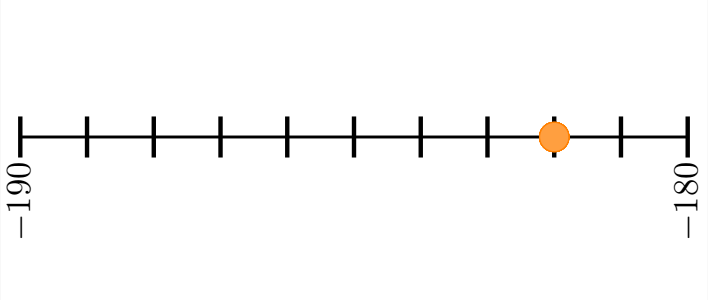
\includegraphics[width=160px]{../images/recta_num_-182.png} \\[-0.5em]   \fillin[$-182$][1.5in]
                        \part 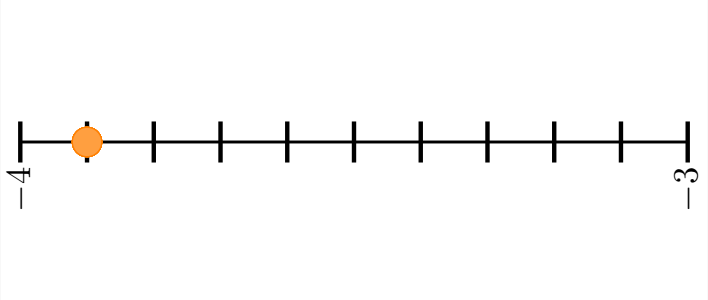
\includegraphics[width=160px]{../images/recta_num_-3.9.png} \\[-0.5em]  \fillin[$-3.9$][1.5in]
                        \part 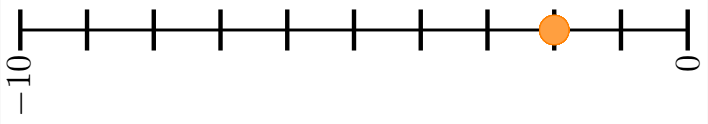
\includegraphics[width=160px]{../images/recta_num_-2.png}  \\[-0.5em]  \fillin[$-2$][1.5in]
                        \part 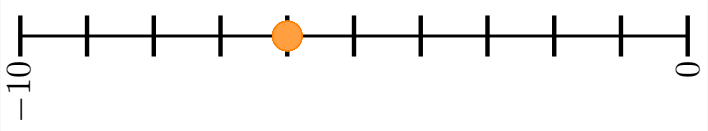
\includegraphics[width=160px]{../images/recta_num_-6.png} \\[-0.5em]  \fillin[$-6$][1.5in]
                        \part 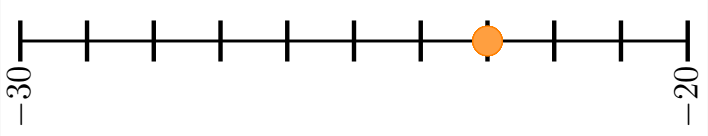
\includegraphics[width=160px]{../images/recta_num_-23.png} \\[-0.5em]  \fillin[$-23$][1.5in]
                        \part 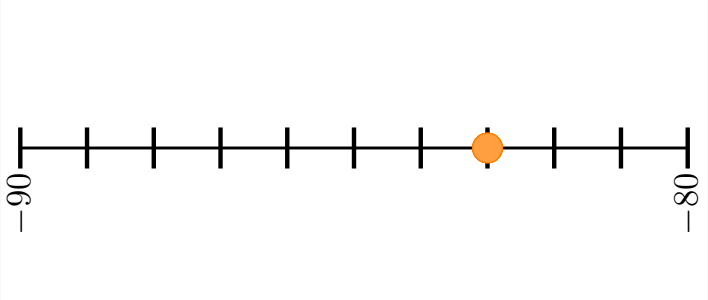
\includegraphics[width=160px]{../images/recta_num_-83.png} \\[-0.5em]  \fillin[$-83$][1.5in]
                  \end{parts}
            \end{multicols}
      }

      \subsection*{\ifprintanswers{Comparación de negativos}\else{}\fi}
      \questionboxed[4]{Escribe sobre la línea el símbolo de mayor que ($>$), menor que ($<$), o igual ($=$) según corresponda.
            \begin{multicols}{2}
                  \begin{parts}\large
                        \part $-182$ \fillin[$>$][0.5in] $-189$
                        \part $-97$ \fillin[$<$][0.5in] $-96.2$
                        \part $-3.9$ \fillin[$>$][0.5in] $-4.1$
                        \part $-0.5$ \fillin[$<$][0.5in] $-0.4$
                        \part $-1.2$ \fillin[$<$][0.5in] $-1.02$
                        \part $-0.5$ \fillin[$>$][0.5in] $-0.6$
                  \end{parts}
            \end{multicols}
      }

      \subsection*{\ifprintanswers{Determina el signo}\else{}\fi}
      \questionboxed[4]{Determina el signo \textit{positivo} o \textit{negativo} que resulta de las siguientes operaciones:
            \begin{multicols}{2}
                  \begin{parts}
                        \part $-28-19$  % \fillin[Negativo][1in]

                        \begin{oneparcheckboxes}
                              \choice Positivo
                              \CorrectChoice Negativo
                        \end{oneparcheckboxes}

                        \part $-43+55$   %\fillin[Positivo][1in]

                        \begin{oneparcheckboxes}
                              \CorrectChoice Positivo
                              \choice Negativo
                        \end{oneparcheckboxes}

                        \part $-223-67$   %\fillin[Negativo][1in]

                        \begin{oneparcheckboxes}
                              \choice Positivo
                              \CorrectChoice Negativo
                        \end{oneparcheckboxes}

                        \part $-23+81$   %\fillin[Positivo][1in]

                        \begin{oneparcheckboxes}
                              \CorrectChoice Positivo
                              \choice Negativo
                        \end{oneparcheckboxes}

                        \part $74-67$  % \fillin[Positivo][1in]

                        \begin{oneparcheckboxes}
                              \CorrectChoice Positivo
                              \choice Negativo
                        \end{oneparcheckboxes}

                        \part $44-80$   %\fillin[Negativo][1in]

                        \begin{oneparcheckboxes}
                              \choice Positivo
                              \CorrectChoice Negativo
                        \end{oneparcheckboxes}

                        \part $87-67$  % \fillin[Positivo][1in]

                        \begin{oneparcheckboxes}
                              \CorrectChoice Positivo
                              \choice Negativo
                        \end{oneparcheckboxes}

                        \part $-105+95$  % \fillin[Negativo][1in]

                        \begin{oneparcheckboxes}
                              \choice Positivo
                              \CorrectChoice Negativo
                        \end{oneparcheckboxes}
                  \end{parts}
            \end{multicols}
      }

      \subsection*{\ifprintanswers{Suma y resta con negativos }\else{}\fi}
      \questionboxed[4]{Realiza las siguientes operaciones con números negativos:
            \begin{multicols}{2}
                  \begin{parts}
                        \part $-28+19=$ \fillin[$-9$][0in]
                        \part $-43-55=$ \fillin[$-98$][0in]
                        \part $-223+67=$ \fillin[$-156$][0in]
                        \part $-23+67=$ \fillin[$44$][0in]
                        \part $(16)-(-14)=$ \fillin[$30$][0in]
                        \part $-23-(-67)=$ \fillin[$44$][0in]
                        \part $-74-(-67)=$ \fillin[$-7$][0in]
                        \part $-44-(-80)=$ \fillin[$36$][0in]
                  \end{parts}
            \end{multicols}
      }
\end{questions}
\end{document}